\chapter{Resultados}
\section{Descripción del experimento}
	Como este documento es una tesis de tipo experimental, las validaciones de la hipótesis deben obtenerse de caracter cuantitativo con una prueba empírica. Una forma de hacerlo es implementando el análisis de los datos de las mediciones de posición dentro del sistema embebido, en este caso el robot humanoide. De esta misma forma, se puede hacer dicha implementación desarrollando la prueba del \textit{RoboCup} llamada \textit{kick from a moving ball}, la cual consiste en patear un balón en movimiento.

	En primera instancia, se tuvo que hacer un desarrollo del sistema de visión del robot, para el robot en físico se tuvo que hacer un nodo que se conecte con el sistema a bajo nivel del hardware de la cámara y publique la imagen 30 veces por segundo en un tópico, para el robot simulado se requirió instalar un \textit{plug-in} dentro del archivo de configuración del robot (.xml) para que sea capaz de simular una cámara y visualice lo que se encuentra dentro del ambiente de Gazebo, véase la Figura: \ref{fig:gazebo}.

	Teniendo ya el sistema de visión con su respectivo procesamiento de imagenes para el posicionamiento del balón se procedió a alimentar al estimador de Kalman con los valores calculados de posición con una doble finalidad, la primera de filtrar el ruido inerente a la medición y la segunda hacer una estimación a \textit{posteriori} de la posición del balón con un limitado número de muestras, dado que si se toman muchas mediciones, podría no dar tiempo para que el robot alcance a patear el balón.
	
	Una vez dejando que el estimador de Kalman logre estimar la posición más probable del balón en un tiempo $t$ el programa espera a que se cumpla cierto umbral de tiempo para comenzar a realizar el movimiento de pateo. Teniendo como objetivo que el pie llegue a una posición determinada por donde va a pasar el balón en movimiento, lo patee y el regrese a su posición inicial. En la Figura \ref{fig:estimator_graphics} se ve cómo es que funciona la prueba completa.
	
\section{Parámetros del experimento}
	La cámara simulada dentro de Gazebo tendrá un rango de visión horizontal estandar que viene por defecto en el \textit{plug-in} de $1.396$ $ rads$ u $80^o$ con una resolución de imagen de 640x480 que es más que suficiente para este experimento. Se consideró suficiente que cada imagen se publique a una frecuencia de 30Hz (un rango cercano al sistema óptico del ser humano), de esta manera le da tiempo al estimador de tomar las muestras necesarias para una oportuna predicción.

	Para que se tenga el mayor rango posible de velocidades del balón en este experimento se requiere hacer que el movimiento de pateo se concluya en el menor tiempo posible, sin embargo, si se le deja poco tiempo para patear, la estabilidad del robot puede verse afectada e incluso peligrosa (más evidentemente para el robot en físico) por lo que se decidió que un tiempo óptimo para patear el balón en un pequeño rango de movimiento es de 0.1 segundos. Con este tiempo se pueden hacer pruebas con una ventana de velocidades del balón de entre 2.0 a 2.8 $m/s$ ya que si es menor el valor, el balón se detiene antes de llegar a la meta esperada y si es mayor, el estimador no tendrá tiempo de hacer el proceso de estimación antes de que el balón sobrepase la meta.
	
	Al principio del experimento el balón tiene una distancia aproximada del robot de 1.2 metros en $y$, se decidió que estuviera a esa distancia debido a que en esa posición está fuera del rango de visión del robot que está esperando recibir la instrucción de patear. Es importante que se mantenga fuera del rango de visión para que cuando detecte una posición del balón, comience a tomar un determinado número de muestras para la predicción de posición. La determinación del número de muestras se hizo de manera empírica con base en los resultados de predicción y corrección. 
	En las  Figuras \ref{fig:estimator_graphic_1}, \ref{fig:estimator_graphic_2} y \ref{fig:estimator_graphic_3} se puede observar que a distintas velocidades (2.5, 3.2 y 3.5 m/s respectivamente) los datos de estimación de Kalman empiezan a converger alrededor de las ocho primeras muestras, por lo que se consideró que son suficientes para que se pueda realizar una predicción confiable.	
	
\begin{figure}
\centering
	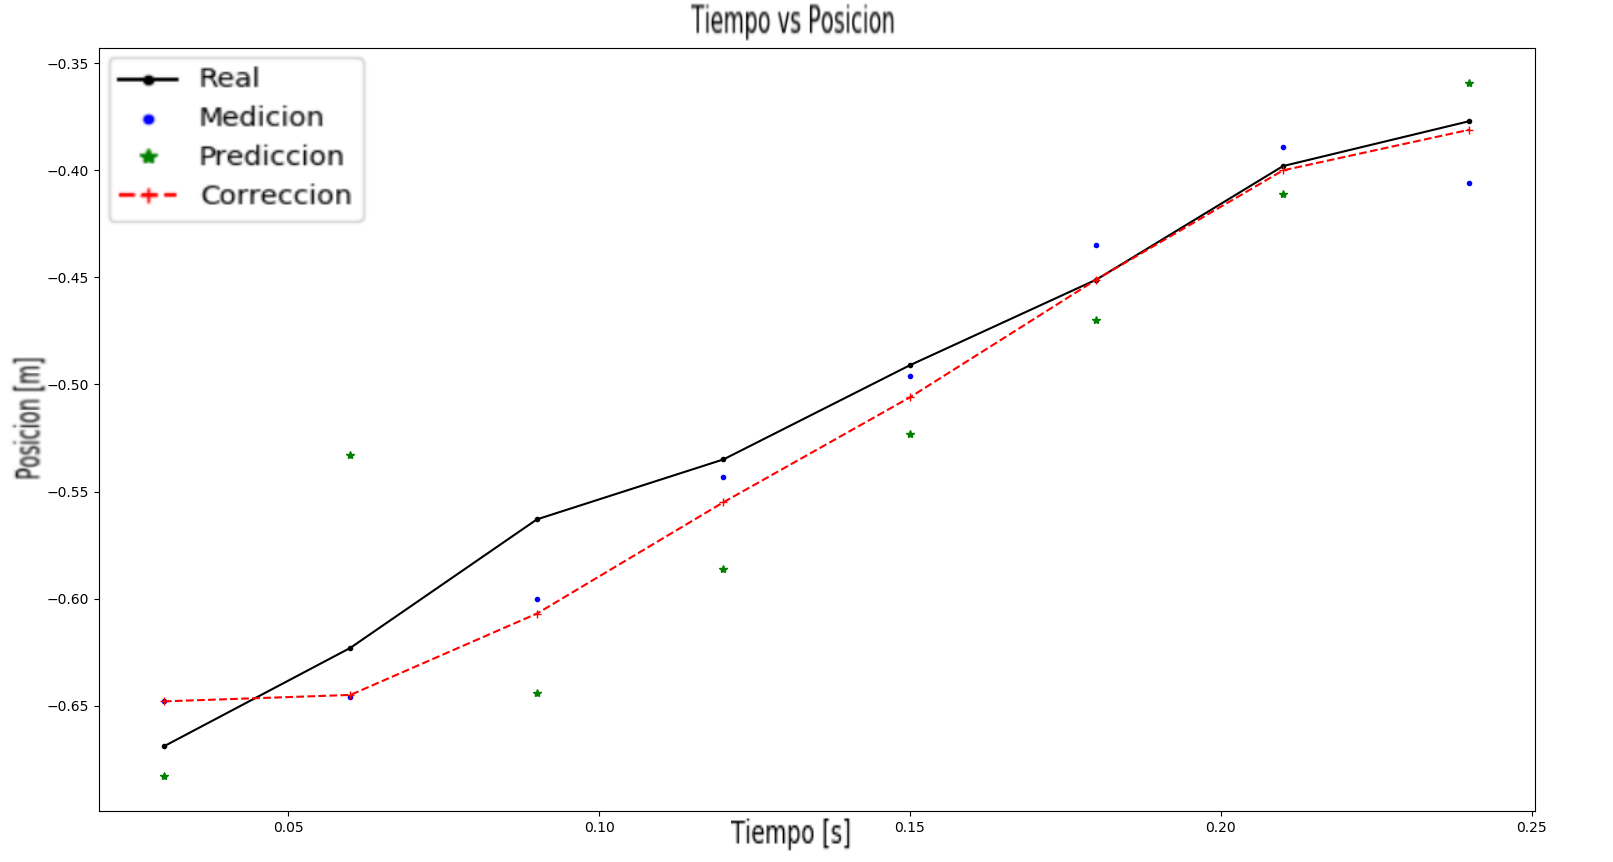
\includegraphics[scale=0.3]{images/test_vel_2dot5.png}
	\caption{Gráfica de tiempo contra posición del balón con una velocidad inicial de 2.5 m/s.}
\label{fig:estimator_graphic_1}
\end{figure}

\begin{figure}
\centering
	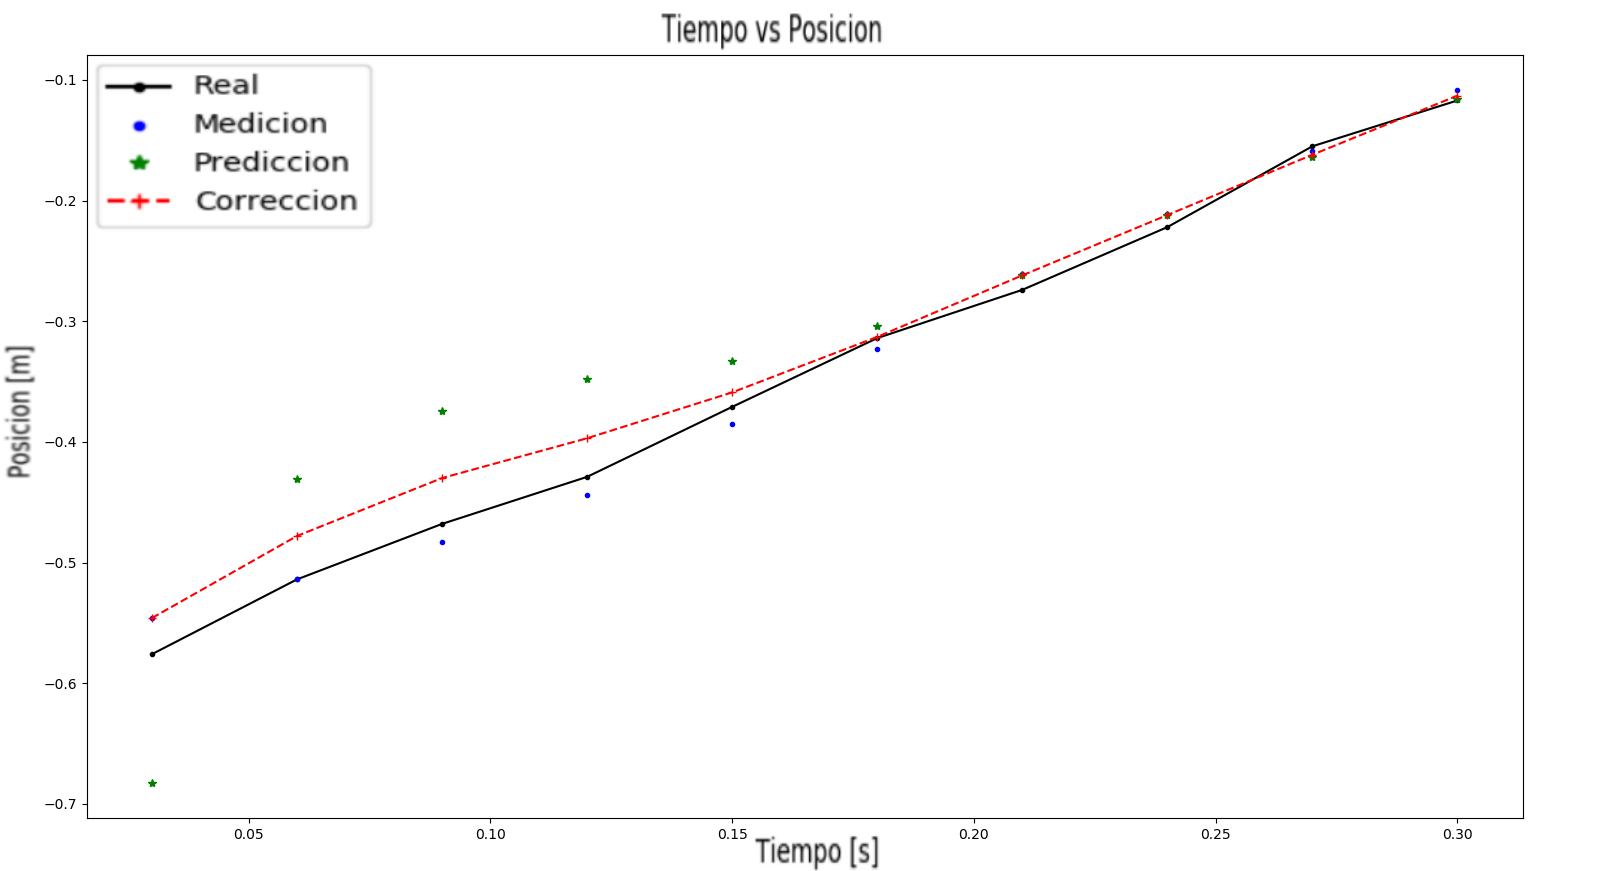
\includegraphics[scale=0.3]{images/test_vel_3dot2.png}
	\caption{Gráfica de tiempo contra posición del balón con una velocidad inicial de 3.2 m/s.}
	\label{fig:estimator_graphic_2}
\end{figure}

\begin{figure}
\centering
	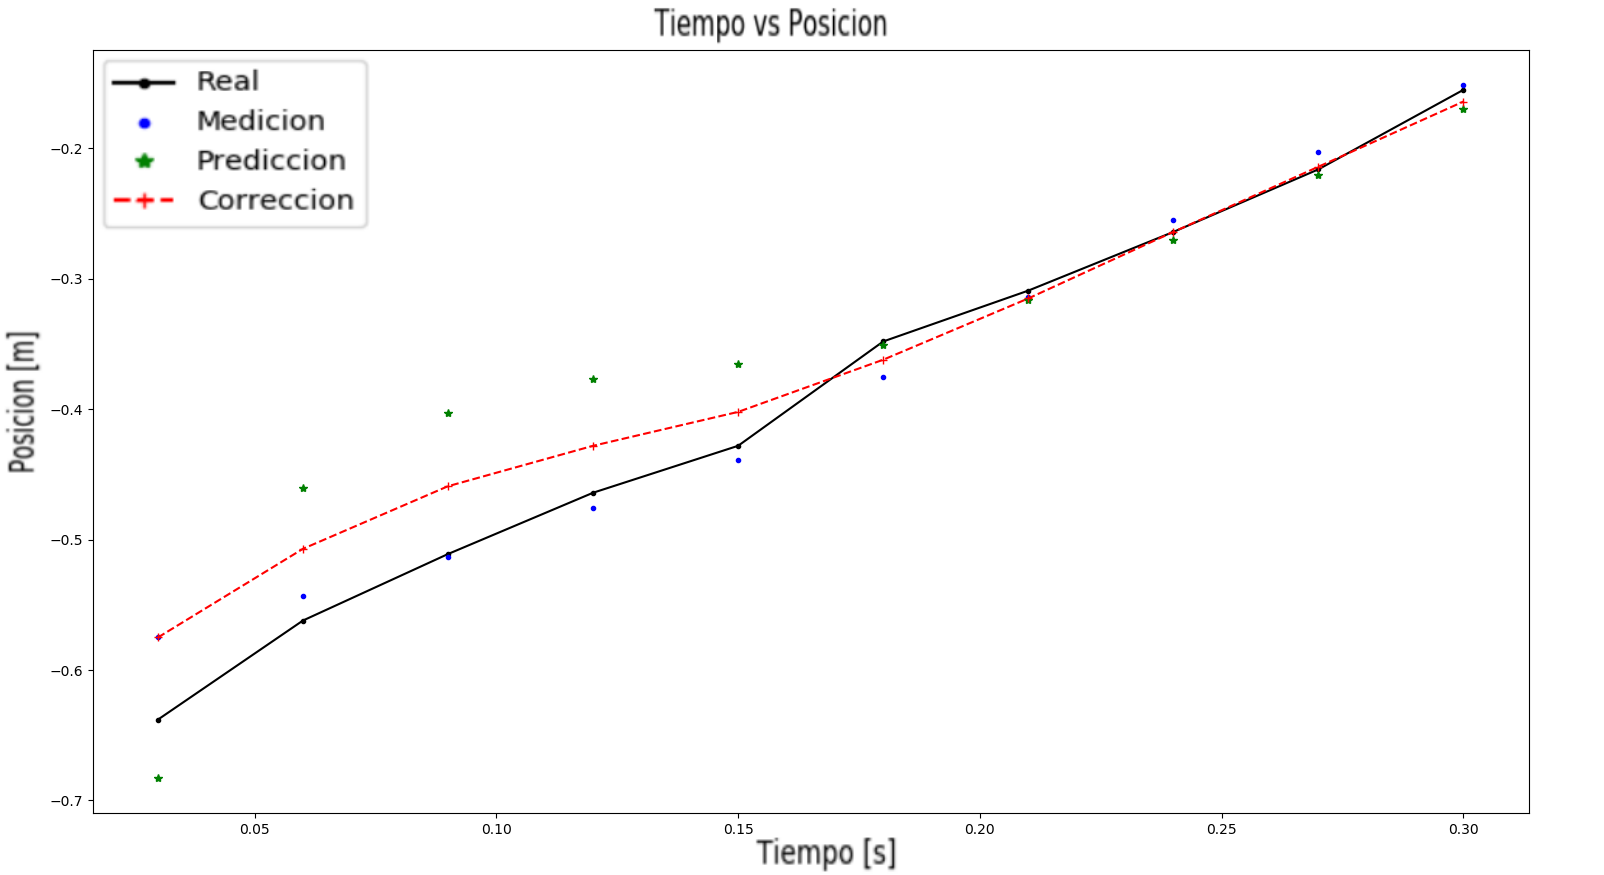
\includegraphics[scale=0.3]{images/test_vel_3dot5.png}
	\caption{Gráfica de tiempo contra posición del balón con una velocidad inicial de 3.5 m/s.}	
	\label{fig:estimator_graphic_3}
\end{figure}
	
	\section{Pruebas de estimación de posición y velocidad}
	La Figura \ref{fig:final_test} se muestra sólo una de varias pruebas que se hicieron en la simulación, variando diversos parámetros para verificar la robustez del sistema de visión y de estimación, entre los principales fueron las velocidades iniciales del balón en movimiento, los ángulos de posición de la cabeza de robot, distancias de recorrido del balón y los coeficientes de fricción dinámica del balón con la superficie.
	
	En la sección 4.3 se obtuvo de manera experimental el coeficiente de fricción dinámica del balón sobre una superficie de fieltro la cual se planea usar para hacer pruebas con el robot real, sin embargo en las pruebas simuladas se fueron observando los diversos comportamientos con coeficientes de ficción menores (desde 0.1 hasta 0.3636) para tener un movimiento más parecido al rectilíneo uniforme. No obstante las pruebas con el coeficiente de fricción obtenido experimentalmente no representaron problemas a la hora de hacer la estimación y se concluyeron los mismos resultados de la prueba de pateo. 
	
\begin{figure}
\centering
	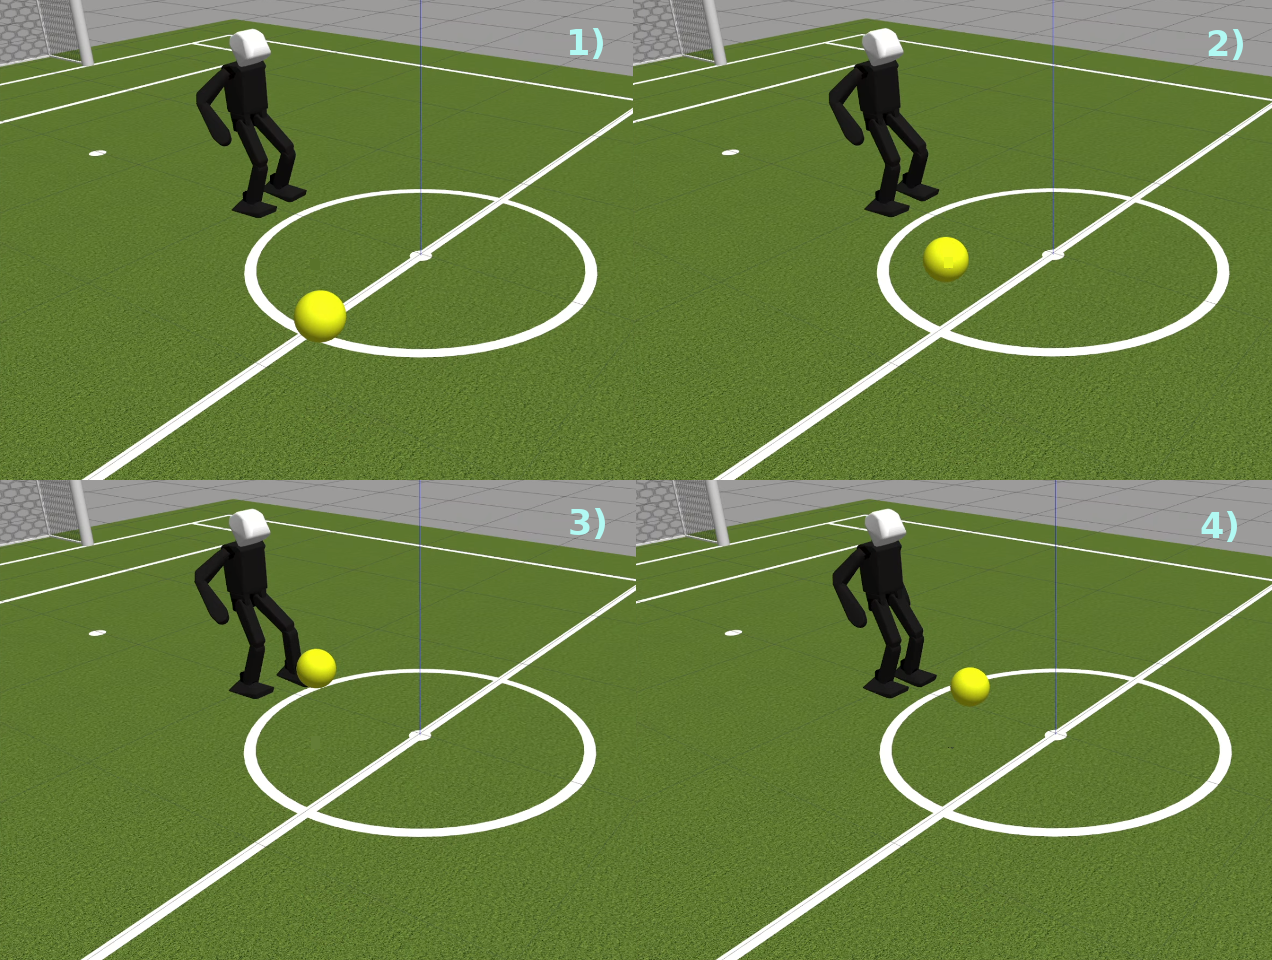
\includegraphics[scale=0.26]{images/final_test.png}
	\caption{Secuencia que ilustra el pateo del balón en movimiento como implementación del filtro.}
\label{fig:final_test}
\end{figure} 